\documentclass[12pt]{article}
\usepackage{amsmath}
\usepackage{lettrine}
\usepackage{amsfonts}
\usepackage{hyperref}
\usepackage[utf8]{inputenc}
\usepackage[english]{babel}
\usepackage{bbm}
\newtheorem{remark}{Remark} 
\newtheorem{theorem}{Theorem}[section]
\newtheorem{corollary}{Corollary}[theorem]
\newtheorem{lemma}[theorem]{Lemma}
\usepackage{tikz}
\usetikzlibrary{decorations.markings}
\usetikzlibrary{arrows}
\graphicspath{
{C:/Users/NitaysLapTop/Documents/MastersDegree/Thesis/DAPHNA_JOEL/Results/Pics/}
}
\newcommand{\maleProb}{\frac{\varepsilon}{\delta + \varepsilon}}

\newcommand{\femaleProb}{\frac{\delta}{\delta + \varepsilon}}

\newcommand{\malellk}{\frac{1}{\sqrt{2\pi}\sigma}e^{-\frac{\big(x - (\mu + \delta)\big)^2}{2\sigma^2}}}

\newcommand{\femalellk}{\frac{1}{\sqrt{2\pi}\sigma}e^{-\frac{\big(x - (\mu - \varepsilon)\big)^2}{2\sigma^2}}}

\newcommand{\purellk}{\frac{1}{\sqrt{2\pi}\sigma}e^{-\frac{\big(x - \mu \big)^2}{2\sigma^2}}}

\title{Estimating KLD for log normal mixture model}

\begin{document}
\maketitle
In this paper I'll present a method to estimate KLD for mixture model of log-normal distribution, relevant for the brain research conducted by prof. Daphna Yoel.
\section{The model}
Our goal is to compute the KLD for both men and women populations. Our model assumes the following:
	\begin{enumerate}
		\item The total mean is 0
		\item The total variance is 1 
		\item The population is composed of equal number of men and women
	\end{enumerate}
The null hypothesis (pure types) assumes the following conditional distributions:
\begin{gather}
f_{men} = \mathcal{N}(\xi, \sigma^2) \\
f_{women} = \mathcal{N}(-\xi, \sigma^2) 
\end{gather}
and $\sigma^2 = 1 - \xi^2$.
The alternative hypothesis (mixture model) assumes the following conditional distributions:
\begin{gather}
f_{men} = p * \mathcal{N}(\xi + \varepsilon, \sigma^2) + (1-p) * \mathcal{N}(\xi - \delta, \sigma^2) \\
f_{women} =  q * \mathcal{N}(\xi + \varepsilon, \sigma^2) + (1-q) * \mathcal{N}(\xi - \delta, \sigma^2) \\
\varepsilon, \delta > 0
\end{gather}
where $p,q$ are the solution to the first assumption:
\begin{gather*}
p * (\xi + \varepsilon) + (1-p) * (\xi - \delta) = \xi \\
q * (\xi + \varepsilon) + (1-q) * (\xi - \delta) = -\xi \\
\end{gather*}
solving the equation system yields:
\begin{gather*}
p = \frac{\delta}{\varepsilon + \delta} \\
q = \frac{\delta - 2 * \xi}{\varepsilon + \delta}
\end{gather*}
with the additional constraint:
\begin{equation}
p,q > 0 \implies \delta > 2 * \xi 
\end{equation}

Next, to satisfy the second assumption we set:
\begin{equation}
  \sigma^2 = 1 - (\xi - \delta)^2 - ((\xi + \varepsilon)^2 - (\xi - \delta)^2) * \frac{p + q}{2}
  \end{equation}  
Since $\sigma^2 > 0 \implies (\xi - \delta)^2 - ((\xi + \varepsilon)^2 - (\xi - \delta)^2) * \frac{p + q}{2} < 1$  
solving this equation yield another constraint:
\begin{equation}
1 > (\xi - \delta)^2 * (1 - \frac{p+q}{2}) + (\xi + \varepsilon)^2 * (\frac{p+q}{2})
\end{equation}
Setting $p,q$ into the last equation yields:
\begin{equation}
(\xi - \delta)^2(2\varepsilon + \xi ^2) + (\xi + \varepsilon)^2(2\delta - \xi ^2) < 2(\varepsilon + \delta)
\end{equation}
\section{KLD computation}
We estimate KLD using Monte Carlo simulation in the following manner. First we sample $n$ observations from the mixture model distribution. Next we compute the likelihood under each scenario:
\begin{gather}
llk_{H_0} = log(\mathcal{N}(\bar{x}, s^2)) \\
llk_{H_1} = log(p_1 * \mathcal{N}(\xi - \delta, \sigma^2) + (1- p_1)* \mathcal{N}(\xi - \varepsilon, \sigma^2))
\end{gather}  	 
To compute KLD we use numeric integration:
\begin{equation}
KLD = \int_{-\infty}^{\infty}log(\frac{f_1(x)}{f_0(x)})f_1(x)dx
\end{equation}
We use the KLD to estimate the set of parameters $\{\xi,\delta,\varepsilon\}$ that a llrt will yield a 50\% power.
\section{Results}
In general the results of the computation draw a picture similar top the one we saw on the first simulation. A ridge like manifold of the KLD over the parameter set. The manifold follows an exponential like curve that peaks at the end of the feasible set at 0.2. 

As we can see, this implies that a sample size of 20K is needed to make a discovery in this region.
\subsection{Feasible parameter set}
One thing worth mentioning is that the results reported above are partially due to the feasible set constraints. The following plot present the feasible set. 

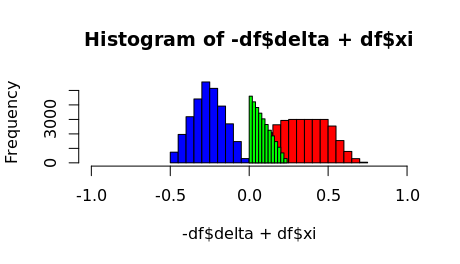
\includegraphics[scale=1]{distribution_of_means.png}  
we can see that the feasible set define a family of mixture models that can be classified into families.
\section{Conclusions and Discussion}
The first conclusion we draw is that the mixture model is hard to detect when the centers are relatively close. We can only make a discovery when the centers are far away. This strengthen the motivation to use the non standardize data and use log-normal distribution.

\subsection*{Discussion}
We need to keep exploring the KLD computation - %TODO: talk with Isaco 
\end{document} 